\documentclass[journal,12pt,twocolumn]{IEEEtran}

\usepackage{setspace}
\usepackage{gensymb}

\singlespacing


\usepackage[cmex10]{amsmath}

\usepackage{amsthm}

\usepackage{mathrsfs}
\usepackage{txfonts}
\usepackage{stfloats}
\usepackage{bm}
\usepackage{cite}
\usepackage{cases}
\usepackage{subfig}

\usepackage{longtable}
\usepackage{multirow}

\usepackage{enumitem}
\usepackage{mathtools}
\usepackage{steinmetz}
\usepackage{tikz}
\usepackage{circuitikz}
\usepackage{verbatim}
\usepackage{tfrupee}
\usepackage[breaklinks=true]{hyperref}
\usepackage{graphicx}
\usepackage{tkz-euclide}
\usepackage{float}

\usetikzlibrary{calc,math}
\usepackage{listings}
    \usepackage{color}                                            %%
    \usepackage{array}                                            %%
    \usepackage{longtable}                                        %%
    \usepackage{calc}                                             %%
    \usepackage{multirow}                                         %%
    \usepackage{hhline}                                           %%
    \usepackage{ifthen}                                           %%
    \usepackage{lscape}     
\usepackage{multicol}
\usepackage{chngcntr}

\DeclareMathOperator*{\Res}{Res}

\renewcommand\thesection{\arabic{section}}
\renewcommand\thesubsection{\thesection.\arabic{subsection}}
\renewcommand\thesubsubsection{\thesubsection.\arabic{subsubsection}}

\renewcommand\thesectiondis{\arabic{section}}
\renewcommand\thesubsectiondis{\thesectiondis.\arabic{subsection}}
\renewcommand\thesubsubsectiondis{\thesubsectiondis.\arabic{subsubsection}}


\hyphenation{op-tical net-works semi-conduc-tor}
\def\inputGnumericTable{}                                 %%

\lstset{
%language=C,
frame=single, 
breaklines=true,
columns=fullflexible
}
\begin{document}
\newtheorem{theorem}{Theorem}[section]
\newtheorem{problem}{Problem}
\newtheorem{proposition}{Proposition}[section]
\newtheorem{lemma}{Lemma}[section]
\newtheorem{corollary}[theorem]{Corollary}
\newtheorem{example}{Example}[section]
\newtheorem{definition}[problem]{Definition}

\newcommand{\BEQA}{\begin{eqnarray}}
\newcommand{\EEQA}{\end{eqnarray}}
\newcommand{\define}{\stackrel{\triangle}{=}}
\bibliographystyle{IEEEtran}
\providecommand{\mbf}{\mathbf}
\providecommand{\pr}[1]{\ensuremath{\Pr\left(#1\right)}}
\providecommand{\qfunc}[1]{\ensuremath{Q\left(#1\right)}}
\providecommand{\sbrak}[1]{\ensuremath{{}\left[#1\right]}}
\providecommand{\lsbrak}[1]{\ensuremath{{}\left[#1\right.}}
\providecommand{\rsbrak}[1]{\ensuremath{{}\left.#1\right]}}
\providecommand{\brak}[1]{\ensuremath{\left(#1\right)}}
\providecommand{\lbrak}[1]{\ensuremath{\left(#1\right.}}
\providecommand{\rbrak}[1]{\ensuremath{\left.#1\right)}}
\providecommand{\cbrak}[1]{\ensuremath{\left\{#1\right\}}}
\providecommand{\lcbrak}[1]{\ensuremath{\left\{#1\right.}}
\providecommand{\rcbrak}[1]{\ensuremath{\left.#1\right\}}}
\theoremstyle{remark}
\newtheorem{rem}{Remark}
\newcommand{\sgn}{\mathop{\mathrm{sgn}}}
\providecommand{\abs}[1]{\vert#1\vert}
\providecommand{\res}[1]{\Res\displaylimits_{#1}} 
\providecommand{\norm}[1]{\lVert#1\rVert}
%\providecommand{\norm}[1]{\lVert#1\rVert}
\providecommand{\mtx}[1]{\mathbf{#1}}
\providecommand{\mean}[1]{E[ #1 ]}
\providecommand{\fourier}{\overset{\mathcal{F}}{ \rightleftharpoons}}
%\providecommand{\hilbert}{\overset{\mathcal{H}}{ \rightleftharpoons}}
\providecommand{\system}{\overset{\mathcal{H}}{ \longleftrightarrow}}
	%\newcommand{\solution}[2]{\textbf{Solution:}{#1}}
\newcommand{\solution}{\noindent \textbf{Solution: }}
\newcommand{\cosec}{\,\text{cosec}\,}
\providecommand{\dec}[2]{\ensuremath{\overset{#1}{\underset{#2}{\gtrless}}}}
\newcommand{\myvec}[1]{\ensuremath{\begin{pmatrix}#1\end{pmatrix}}}
\newcommand{\mydet}[1]{\ensuremath{\begin{vmatrix}#1\end{vmatrix}}}
\numberwithin{equation}{subsection}
\makeatletter
\@addtoreset{figure}{problem}
\makeatother
\let\StandardTheFigure\thefigure
\let\vec\mathbf
\renewcommand{\thefigure}{\theproblem}
\def\putbox#1#2#3{\makebox[0in][l]{\makebox[#1][l]{}\raisebox{\baselineskip}[0in][0in]{\raisebox{#2}[0in][0in]{#3}}}}
     \def\rightbox#1{\makebox[0in][r]{#1}}
     \def\centbox#1{\makebox[0in]{#1}}
     \def\topbox#1{\raisebox{-\baselineskip}[0in][0in]{#1}}
     \def\midbox#1{\raisebox{-0.5\baselineskip}[0in][0in]{#1}}
\vspace{3cm}
\title{ASSIGNMENT 3}
\author{Dishank Jain \\ AI20BTECH11011}
\maketitle
\newpage
\bigskip
\renewcommand{\thefigure}{\theenumi}
\renewcommand{\thetable}{\theenumi}
Download all python codes from 
\begin{lstlisting}
https://github.com/Dishank422/EE3900/blob/main/assignment3_elegant/codes
\end{lstlisting}
%
and latex-tikz codes from 
%
\begin{lstlisting}
https://github.com/Dishank422/EE3900/blob/main/assignment3_elegant/Assignment3.tex
\end{lstlisting}
%
\section{Constructions Q2.4}
Construct a quadrilateral ABCD such that BC = 4.5, AC = 5.5, CD = 5, BD = 7  and AD = 5.5.

\section{Solution}
\begin{lemma}
In triangle XYZ, if the \ref{1}-\ref{5} hold, 
\begin{align}
    XY &= z\label{1}\\
    YZ &= x\label{2}\\
    XZ &= y\label{3}\\
    \vec{X} &= \myvec{0\\0}\label{4}\\
    \vec{Y} &= \myvec{z\\0}\label{5}
\end{align}
then 
\begin{align}
    \vec{Z} &= \myvec{m\\ \pm n}\\
    where\; m &= \dfrac{XY^2+XZ^2-YZ^2}{2\times XY}\\
    n &= \sqrt{(XZ^2-m^2)}
\end{align}
\end{lemma}
Note: The proof for above can be found in the manual (problem 1.3).
Using AC = 5.5,
\begin{align}
    Let\; \vec{A} = \myvec{0\\0},\; &\vec{C} = \myvec{5.5\\0}\\
    \vec{D} = &\myvec{h\\k}
\end{align}

We know 
\begin{align}
    \norm{\vec{D}-\vec{A}} &= 5.5\label{DA}\\
    \norm{\vec{D}-\vec{C}} &= 5\label{DC}\\
    \norm{\vec{B}-\vec{C}} &= 4.5\label{BC}\\
    \norm{\vec{B}-\vec{D}} &= 7\label{BD}
\end{align}
\begin{align}
    h &= \dfrac{AC^2+AD^2-CD^2}{2AC}\\
      &= \dfrac{5.5^2+5.5^2-5^2}{2\times 5.5}\\
      &= 3.23\\
    k &= \sqrt{(AD^2-h^2)}\\
      &= \sqrt{(5.5^2-h^2)}\\
      &= 4.45\\
    \implies \vec{D} &= \myvec{3.23\\4.45}
\end{align}
Note: Above computations can be found in codes/finding\textunderscore D.py.

Now we shall transform co-ordinates of $\vec{C}, \vec{D}$ such that C will become the new origin and $\vec{D}$ comes along the positive x-axis. We shall first shift origin to C. For this, we have to subtract $\myvec{5.5\\0}$ from co-ordinates of $\vec{C}, \vec{D}$.
\begin{align}
    \implies &\vec{C}_1 = \myvec{0\\0}\\
    &\vec{D}_1 = \myvec{-2.27\\4.45}
\end{align}

Next we shall rotate the co-ordinates such that $\vec{D}_1$ is on the x-axis. For this, we have to multiply the co-ordinates with the clockwise rotator matrix $\vec{R}$, given as
\begin{align}
    \vec{R} &= \myvec{\cos{\theta}& \sin{\theta}\\ -\sin{\theta} & \cos{\theta}}\\
    where\; \theta &= \arccos{\dfrac{\vec{D}_1\cdot \myvec{1\\0}^\top}{\norm{\vec{D}_1}}}\\
    &= \arccos{\dfrac{-2.27}{5}}\\
    &= 2.04 \;radians\\
    \implies \vec{R} &= \myvec{-0.45 & 0.89\\-0.89 & -0.45}\\
    \implies \vec{D}_2 &= \vec{R}\vec{D}_1 = \myvec{5\\0}
\end{align}
Note: norm of $\vec{D}$ is calculated using codes/norm\textunderscore D1.py, arccos is calculated using codes/finding\textunderscore theta.py, R is calculated using codes/R.py and $\vec{D}_2$ is calculated using D2.py.

Since $\vec{C}_1$ is origin
\begin{equation}
    \vec{C}_2 = \vec{C}_1
\end{equation}
\begin{equation}
    Let\; \vec{B}_2 = \myvec{p\\q}
\end{equation}

Using \ref{BC} and \ref{BD},
\begin{align}
    \norm{\vec{B}_2-\vec{C}_2} &= 4.5\\
    \norm{\vec{B}_2-\vec{D}_2} &= 7
\end{align}
\begin{align}
    p &= \dfrac{B_2C_2^2+C_2D_2^2-B_2D_2^2}{2C_2D_2}\\
      &= \dfrac{4.5^2+5^2-7^2}{2\times 5}\\
      &= -0.38\\
    q &= \pm \sqrt{(B_2C_2^2-p^2)}\\
      &= \pm 4.48\\
    \implies \vec{B}_2 &= \myvec{-0.38\\4.48}, \myvec{-0.38\\-4.48}
\end{align}
Note: q is found using codes/q.py. 

To get $\vec{B}_1$, we operate on $\vec{B}_2$ with inverse of $\vec{R}$. Inverse of $\vec{R}$ is nothing but $\vec{R}(-\theta)$. Therefore,
\begin{align}
    \vec{R}^{-1} &= \myvec{\cos{-\theta}& \sin{-\theta}\\ -\sin{-\theta} & \cos{-\theta}}\\
                 &= \myvec{\cos{\theta}& -\sin{\theta}\\ \sin{\theta} & \cos{\theta}}\\
                 &= \myvec{-0.45 & -0.89\\0.89 & -0.45}\\
    \implies \vec{B}_1 &= \vec{R}^{-1}\vec{B}_2 = \myvec{-3.82\\-2.35}, \myvec{4.16\\1.68}
\end{align}

To finally get $\vec{B}$, we add $\myvec{5.5\\0}$ to $\vec{B}_1$.
\begin{equation}
    \implies \vec{B} = \myvec{1.68\\-2.35}, \myvec{9.66\\1.68}
\end{equation}

We want $\vec{A},\vec{B},\vec{C},\vec{D}$ in clockwise or anti-clockwise order. Therefore only the first value of $\vec{B}$ is possible. 
\begin{equation}
    \implies \vec{B} = \myvec{1.68\\-2.35}
\end{equation}
Using the co-ordinates of the vertices as found, the following quadrilateral is plotted.
\begin{figure}[h]
    \resizebox{\columnwidth}{!}{
    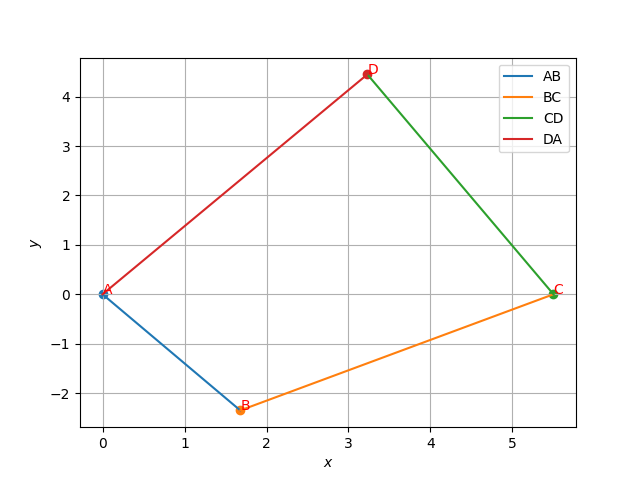
\includegraphics{figures/figure.png}
    }
    %\caption{Required quadrilateral}
    %\label{quad_plot}
\end{figure}
\end{document}
